\documentclass[11pt]{article}

\usepackage[utf8]{inputenc}  
\usepackage{amsmath}         
\usepackage{amssymb}         
\usepackage{graphicx}        
\usepackage{geometry}        
\usepackage{fancyhdr}        
\usepackage{hyperref}       
\usepackage{float} 
\usepackage{xcolor}
\usepackage{ulem}
\usepackage{tabularx}
\usepackage{cancel}
\usepackage{caption}

% Impostazioni per i margini
\geometry{a4paper, margin=0.8in}

% Intestazioni
\pagestyle{fancy}
\fancyhf{}
\fancyhead[L]{Linguaggi Formali e Compilatori 2024/25}
\fancyhead[R]{Codice Intermedio - Array SDT}
\fancyfoot[C]{\thepage}   
\setlength{\headheight}{14pt}

\begin{document}
\section{Considerazioni}
Queste sono piccole note che cercano di ampliare le slide sulla parte 
di generazione codice per le operazioni sugli array. Come dalle slide
si considerreranno array salvati in memoria per \textbf{Row-Major order}.
Ricordo anche che la notazione per il tipo di un array di interi k-dimensionale viene 
denotato:
$$array(size_1, array(size_2, array(...(size_k, int))))$$
\section{Syntax Directed Translation per gli Array}
\subsection{Indirizzamento}
Il problema maggiore nel generare codice per referenziare array sta nel
calcolo degli indirizzi dei suoi elementi, prendiamo l'indirizzo di $A[i]$:
$$base + i \cdot w$$
in cui $base$ è l'indirizzo relativo al primo elemento di $A$ e $w$ è la 
grandezza di ogni elemento dell'array, se volessimo indirizzare l'elemento 
$A[i_1][i_2]$ di una matrice assumendo che $w_1$ è la dimensione di una riga della matrice  e $w_2$ è la dimensione di ogni elemento avremo:
$$base + i_1 \cdot w_1 + i_2 \cdot w_2 $$
In k-dimensioni otteniamo:
\begin{equation} \label{eq:sum-offset}
  base + i_1\cdot w_1 + i_2 \cdot w_2 + \dots + i_k \cdot w_k
\end{equation}
\subsection{Grammatica}
Consideriamo la seguente grammatica in cui $E$ rappresenta delle espressioni 
mentre $L$ rappresenta il nome di un array (quindi la sua locazione in memoria):
$$S \rightarrow id = E\;|\;L = E $$
$$E \rightarrow id \; |\; L \;|\; E + E$$
$$L \rightarrow id[E] \; |\; L[E]$$
Da questa grammatica possiamo generare ad esempio:
\begin{figure}[!htb]
  \centering
  \minipage{0.32\textwidth}
    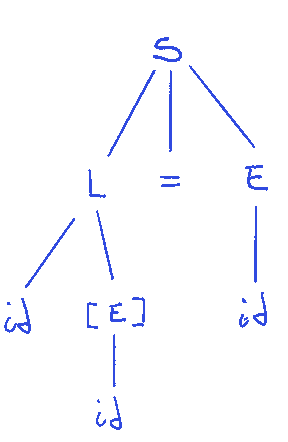
\includegraphics[width=\linewidth, height=3cm, keepaspectratio]{img/DerivationTree0.png}
    \caption*{$a[b] = c$}\label{fig:derivation-tree-0}
  \endminipage\hfill
  \minipage{0.32\textwidth}
    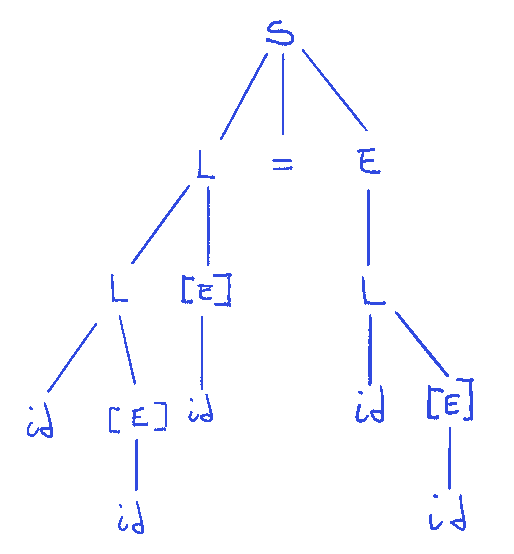
\includegraphics[width=\linewidth, height=3cm, keepaspectratio]{img/DerivationTree1.png}
    \caption*{$a[b][c]=d[e]$}\label{fig:derivation-tree-1}
  \endminipage\hfill
  \minipage{0.32\textwidth}
    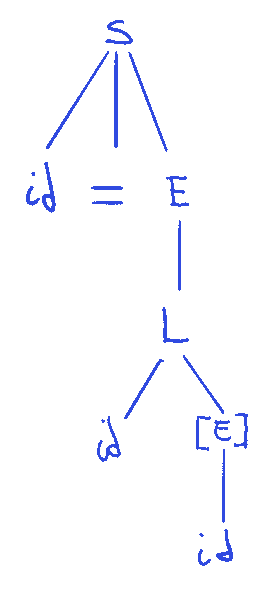
\includegraphics[width=\linewidth, height=3cm, keepaspectratio]{img/DerivationTree2.png}
    \caption*{$a = b[c]$}\label{fig:derivation-tree-2}
  \endminipage
\end{figure}

\subsection{Attributi}
\begin{itemize}
  \item $L.addr$ denota un temporaneo che viene usato per calcolare l'indirizzo
  dell'elemento dell'array sommando i termini $i_j \cdot w_j$ in (\ref{eq:sum-offset})
  \item $L.array$ è un puntatore ad una entry della tabella dei simboli per il
  nome dell'array, in cui $L.array.base$ rappresenta l'indirizzo base dell'array
  \item $L.type$ è il tipo del sotto array generato da $L$, per ricavare il tipo
  utilizzeremo $arg2$ che va a recuperare il secondo argomento (per esempio 
  $arg2(2, array(3, int))=array(3, int)$)
  \item $L.width$ é la grandezza del subarray generato da $L$, ricavata attraverso 
  la funzione ausiliaria $width()$ (per esempio $width(array(3, int)) = 3 \cdot int_{size}$) 
\end{itemize}
\subsection{Regole semantiche}
La produzione $\mathbf{S \rightarrow id = E}$ deve generare il codice di assegnamento a 
una variabile con il valore di un'espressione: 
$$\{gen(table.get(id) \;'\mathord{=}'\; E.addr);\}$$
Le azioni semantiche per $\mathbf{S \rightarrow L=E}$ devono generare il codice che assegna
il valore dell'espressione \textbf{E} alla locazione di memoria referenziata da \textbf{L}. 
\\Ricordando che: 
\begin{itemize}
  \item $L.array$ è il puntatore all'array nella tabella dei simboli
  \item $L.array.base$ è l'indirizzo del primo elemento
  \item $L.addr$ denota il temporaneo che contiene l'offset dell'elemento
\end{itemize}
possiamo concludere che l'elemento sarà in $L.array.base[L.addr]$ e l'istruzione generata 
copierà r-value da $E.addr$ alla locazione di L:
$$\{gen(L.array.base\;'\,[\,'\;L.addr\;'\,]\,'\;'\mathord{=}'\; E.addr);\}$$
Le produzioni $\mathbf{E\rightarrow E_1+E_2}$ e per $\mathbf{E\rightarrow id}$ sono analoghe 
alla prima:
$$\{gen(E.addr \;'\mathord{=}'\; E_1.addr \;'\mathord{+}'\; E_2.addr );\}$$
$$\{gen(E.addr \;'\mathord{=}'\; table.get(id) );\}$$
La produzione $\mathbf{E\rightarrow L}$ deve generare il codice per copiare l'elemento dell'array 
denotato da \textbf{L} in un nuovo temporaneo:
$$\{E.addr = newTemp();\quad gen(E.addr '\mathord{=}' L.array.base\;'['\;L.addr\;']');\}$$
La produzione $\mathbf{L \rightarrow id[E]}$ deve trasferire le informazioni sull'array denotato 
da \textbf{id} in \textbf{L}.



\begin{center}
\begin{tabularx}{\linewidth}{l m{0.6\linewidth}}
$\{L.array = table.get(id);$ 
    & \small Recupera la voce della tabella dei simboli dell'array utilizzando l'identificatore id (ad es., "a") \\[0.3cm]

$L.type = arg2(table.getType(id));$ 
    & \small Estrae il tipo del sottoarray. Ad esempio, se $a$ è $array(2, array(3, integer))$, $L.type$ diventa $array(3, integer)$ \\[0.3cm]

$L.width = width(L.type)$ 
    & \small Determina la dimensione (in byte) del sottoarray rappresentato da $L.type$ \\[0.3cm]

$L.addr = \text{newTemp()}$ 
    & \small Crea un nuovo temporaneo \\ [0.3cm]

$\text{gen}(L.addr \;'\mathord{=}'\;E.addr \;'*'\; L.width\; )\}$ 
    & \small Calcola il primo offset, cioè in $a[i_1][i_2][...] \rightarrow i_1 \cdot w_1$ \\
\end{tabularx}
\end{center}

\noindent Infine la produzione $\mathbf{L \rightarrow L_1[E] }$ dovrà trasferire i dati processati da id,
ed aggiornare l'offset per il corretto indirizzamento dell'elemento:

\begin{center}
  \begin{tabularx}{\linewidth}{l m{0.6\linewidth}}
  $\{L.array = L_1.array$
      & \small L'array a cui si fa riferimento rimane lo stesso. \\[0.3cm]
  
  $L.type = arg2(L_1.type)$
      & \small Estrae il tipo del sottoarray a questo livello. Se $L_1.type$ era array(3, integer), $L.type$ diventa integer. \\[0.3cm]
  
  $ L.width = width(L.type) $
      & \small Calcola la dimensione del sottoarray corrente (ad esempio, la dimensione di un integer).\\[0.3cm]
  
  $ t = \text{newTemp()} $
      & \small Crea un nuovo temporaneo per l'elaborazione intermedia \\[0.3cm]
  
  $ \text{gen}(t \;'\mathord{=}'\; E.addr \;'*'\; L.width)$
      & \small Calcola l'offset per la dimensione corrente (utilizzando $E.addr$ per l'indice e $L.width$) e lo memorizza in una variabile temporanea t. \\[0.3cm]
  
  $ L.addr = \text{newTemp()} $
      & \small Crea un altro temporaneo per l'indirizzo risultante \\[0.3cm]
  
  $ \text{gen}(L.addr \;'\mathord{=}'\; L_1.addr \;'+'\; t )\}$
      & \small Combina l'offset del livello precedente ($L_1.addr$) con l'offset appena calcolato (t) per ottenere l'offset totale per questo elemento. Questo offset totale viene quindi memorizzato in L.addr. \\
  \end{tabularx}  
\end{center}
\end{document}